\chapter{Deep Learning}
\label{cha:dnn}
Deep Learning research in the field of artificial neural networks~(ANNs) has dominated state-of-the-art solutions on cognitive tasks, e.g. the performance exceeding human-level  on image classification tasks~\citep{he2015delving} and playing GO~\citep{silver2016mastering}).
Merging \protect\TLSdel{deep learning} \protect\TLSins{Deep Learning} techniques into SNNs may provide an answer to the problem of how to operate SNNs to perform as well as ANNs in cognitive tasks. 
In this chapter, we will give an overview of popular architectures and models of \protect\TLSdel{deep learning} \protect\TLSins{Deep Learning} in Section~\ref{sec:dl_history}, and the rest of this chapter will illustrate the mechanisms of convolutional networks (ConvNets), autoencoders (AEs), and restricted Boltzmann machines~(RBMs) in detail which will be used in following chapters.

\section{Brief Overview}
\label{sec:dl_history}
Deep \protect\TLSdel{learning} \protect\TLSins{Learning} seems to have become the answer to all artificial intelligence problems overnight since Geoffrey Hinton proposed the training method of a type of ANN, \protect\TLSdel{deep belief network,} \protect\TLSins{the Deep Belief Network,} in 2006~\citep{hinton2006fast}.
However, \protect\TLSdel{deep learning} \protect\TLSins{Deep Learning} is not a new `magic', but rather has a history over a few decades and its sudden success is the result of the availability of an increasing amount of training data, \protect\TLSins{the} growing size of network models and greater computational power.
Therefore, all the classical \protect\TLSdel{deep learning} \protect\TLSins{Deep Learning} architectures date back to the last century \protect\TLSdel{when deep learning un-named.} \protect\TLSins{before the `Deep Learning' named was coined.}
However, at that time, deep networks \protect\TLSdel{were} \protect\TLSins{could} hardly \protect\TLSdel{to} be \protect\TLSdel{trained} \protect\TLSins{trained,} mainly because of the \protect\TLSdel{limit} \protect\TLSins{limits} on computational power.


\subsection{Classical Models}
We call the well-known and widely-used \protect\TLSdel{deep learning} \protect\TLSins{Deep Learning} models `classical' and give a brief introduction to those models in this section. 
As mentioned above, the first break-through \protect\TLSdel{of} \protect\TLSins{in} training deep, \protect\TLSdel{not} \protect\TLSins{as opposed to} shallow ($\le 3$ layers), networks was the greedy layer-wise strategy~\citep{hinton2006fast} proposed to train stacked RBMs, which will be described in more detail in Section~\ref{sec:rbm}.
Shortly after that this method was proved to be efficient for training other kinds of deep networks including stacked AEs~\citep{bengio2007greedy} (stated in Section~\ref{sec:AE}).
RBMs and AEs are suitable for dimensionality reduction and feature extraction when trained with unsupervised learning on unlabelled data.
In 2012, using such \protect\TLSdel{a} \protect\TLSins{an} unsupervised \protect\TLSdel{deep learning architecture} \protect\TLSins{Deep Learning architecture,} the Google Brain team achieved a milestone in the \protect\TLSdel{deep learning} \protect\TLSins{Deep Learning} era; the neural network learned to recognise cats by `watching' 10 million images generated from random frames of YouTube videos~\citep{le2013building}.

ConvNets are biologically inspired from the significant discovery of Hubel and Wiesel that the orientation selectivity (simple cells) and pooling mechanism (complex cells) represent the basic functions in the primary visual cortex in cats~\citep{hubel1962receptive}.
These simple cells fire at a high frequency to their preferred orientation of visual stimuli within their receptive fields~(shown in Figure~\ref{Fig:v1}), small sub-regions of the visual field.
Meanwhile, a complex cell corresponds to the existence of a pattern within a larger receptive field but loses the exact position of the pattern.
\protect\TLSins{The} NeoCognitron~\citep{fukushima1982neocognitron} was the first \protect\TLSins{network} to mimic the functions of V1 simple and complex neurons in an artificial neural network, and later this feature detection of single cells was improved by sharing weights among receptive fields in LeNet-5~\citep{lecun1998gradient}, the typical ConvNet used today.
The mechanism of shared weights forms the essence of convolution in a ConvNet, which hugely reduces the number of weight parameters in a network.
The most significant milestones produced by deep ConvNet dominated the best performances in the annual ImageNet Challenge~\citep{russakovsky2015imagenet}: AlexNet~\citep{krizhevsky2012imagenet}, VGG Net~\citep{simonyan2014very}, GoogLeNet~\citep{szegedy2015going} and ResNet~\citep{he2016deep}.

Despite the powerful capabilities of these feed-forward deep networks, sequence processing is a challenge for them since the input and output vectors are of static size.
Thus recurrent neural networks~(RNNs), containing feed-back connections, are ideal solutions for dealing with sequential information since their current output is always \protect\TLSdel{dependant} \protect\TLSins{dependent} on the previous `memory'.
As training mechanisms have become more mature, for example using the long short-term memory or (LSTM)~\citep{hochreiter1997long}, RNNs have shown great success in many natural language processing tasks: language modelling~\citep{mikolov2010recurrent}, machine translation~\citep{sutskever2014sequence}, speech recognition~\citep{graves2014towards} and image caption generation~\citep{karpathy2015deep}.

\subsection{Combined Approaches}
\protect\TLSdel{Current}
\protect\TLSins{The current} trend \protect\TLSdel{of deep learning} \protect\TLSins{in Deep Learning} is to combine machine learning algorithms towards more complex \protect\TLSdel{objectives:} \protect\TLSins{objectives} such as decision making and data generation.

Reinforcement learning (RL) is inspired from animal behaviour when agents learn to make sequential optimised decisions to control an environment.
To address complex decision making problems in practical life, RL requires a sufficiently abstract representation of the high-dimensional \protect\TLSdel{environment, where deep learning} \protect\TLSins{environment.
Here Deep Learning} is \protect\TLSdel{exactly clever} \protect\TLSins{very effective} at dimensionality reduction and feature extraction.
The milestone achieved by \protect\TLSins{the} integration of RL and deep networks, \protect\TLSdel{the} deep \protect\TLSdel{reinforcement learning,} \protect\TLSins{RL,} drew everyone's attention \protect\TLSdel{on} \protect\TLSins{to} artificial intelligence when AlphaGo beat a professional human player \protect\TLSdel{in} \protect\TLSins{at} Go~\citep{silver2016mastering}.

Generative Adversarial Networks (GANs)~~\citep{goodfellow2014generative} are proposed for training generative models of complex data.
Instead of training discrimination networks (e.g. image classification using CovNets ) and generation networks (e.g. data sampling on RBMs) separately with different objectives, GANs train two competing networks, one the discriminator, the other the generator, simultaneously by continuously using them to play games with each other.
Thus, the generator learns to produce more realistic data to \protect\TLSdel{cheat} \protect\TLSins{fool} the discriminator; meanwhile the discriminator learns to become better at distinguishing generated from real data.
Exciting achievements have been reported \protect\TLSdel{on} \protect\TLSins{in} generating complex data such as realistic image generation based on \protect\TLSdel{description} \protect\TLSins{descriptions} in text~\citep{radford2015unsupervised}.

\section{Convolutional Networks}
\label{sec:convnet}
In Chapter~\ref{cha:Conv}, we will use a convolutional network to demonstrate a training method \protect\TLSdel{on} \protect\TLSins{for} spiking deep architectures.
This section aims to give a detailed introduction to ConvNet architectures and \protect\TLSdel{its} \protect\TLSins{their} training with back propagation.
\subsection{Network Architecture}

	\begin{figure}[bt]
		\centering
		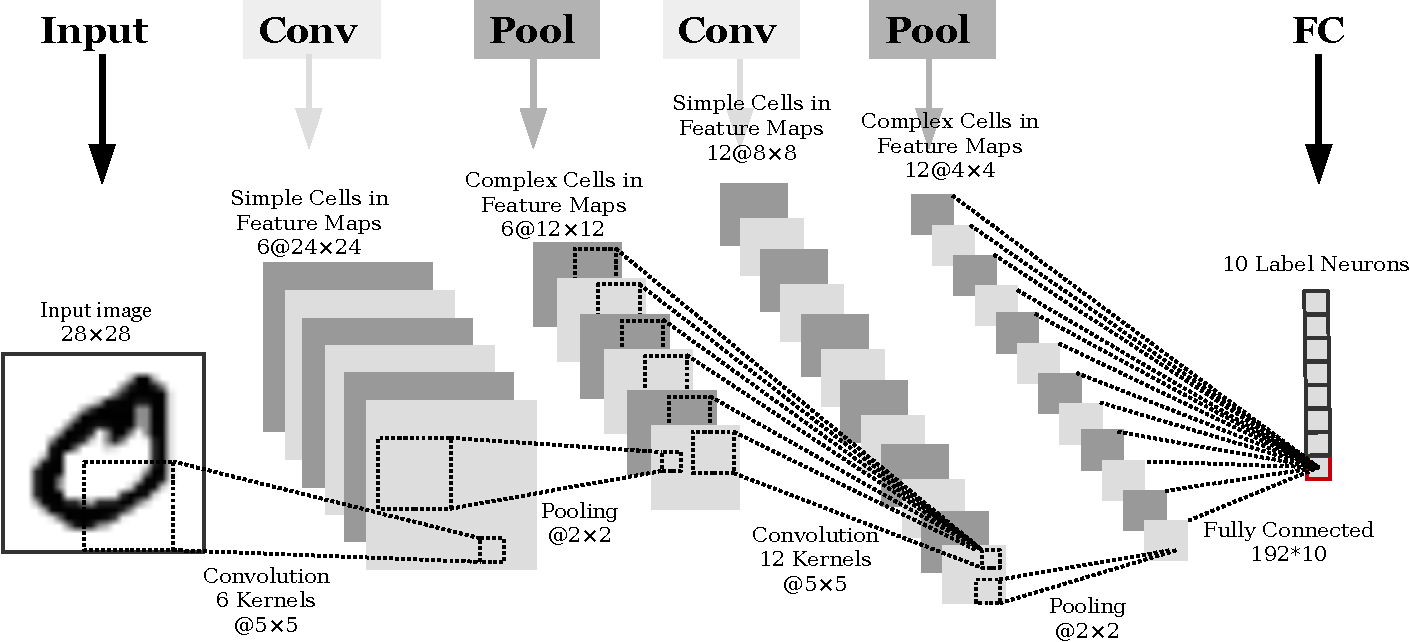
\includegraphics[width=0.95\textwidth]{pics_snn/convnet.pdf}
		\caption{Typical ConvNet architecture.}
		\label{Fig:ConvNet}
	\end{figure}

A typical ConvNet (LeNet) consists of four types of neural layers: an input layer, convolutional~(Conv) layers of simple cells, \protect\TLSdel{pooling} \protect\TLSins{pooling~(Pool)} layers of complex cells and fully-connected~(FC) layers, as shown in Figure~\ref{Fig:ConvNet}.
From the left to right of Figure~\ref{Fig:ConvNet}, we illustrate the mechanism of \protect\TLSins{the} ConvNet in detail.

The pixels of the input image are normalised and fed into the first Conv layer.
Every simple cell takes inputs within its receptive field and the weights on each input pixel are determined by the convolutional kernel which has the same size as the receptive field.
The neurons work as demonstrated in Figure~\ref{Fig:compare_as}(a) performing a dot product between the weights and the input volume of a receptive field; this is followed by an activation function.
Convolving a whole input image with a kernel composes a feature map in the Conv layer, thus there are 6 feature maps in the first Conv layer.
Stride controls the output volume of a convolution such that setting the stride to $step$ causes the kernel \protect\TLSdel{moving} \protect\TLSins{to move} $step$ pixels at a time.
Thus a small stride produces more output volume and highly overlapping receptive fields.
Suppose an input image and a kernel are both squares with side lengths of $l_{in}$ and $l_k$, then the side length of the convolved feature map is $(l_{in} - l_k + 1)/stride$.

The special characteristics of Conv layers lie in the local connectivity and the parameter sharing, such that a neuron connects only to a spatially local input volume, its receptive field; and the weights \protect\TLSdel{(convolutional} \protect\TLSins{(the convolutional} kernel) are shared among all the receptive fields.
Consequently, the number of parameters (trainable weights) hugely decreases compared to all-to-all connections of \protect\TLSins{the} same network size. 

The complex neurons of \protect\TLSdel{pooling} \protect\TLSins{the Pool} layers either output the maximum input within their receptive fields (max pooling) or the \protect\TLSdel{averaging} \protect\TLSins{average} (average pooling), \protect\TLSdel{as} \protect\TLSins{by} applying a max/average filter to non-overlapping receptive fields.
The pooling process reduces the spatial size of the feature maps but keeps the number of features.
In Chapter~\ref{cha:Conv}, we will use average pooling of $2\times2$ for all the \protect\TLSdel{pooling} \protect\TLSins{Pool} layers, \protect\TLSins{as} shown in Figure~\ref{Fig:ConvNet}.
The average filter traverses \protect\TLSdel{over} an entire feature map with a stride of 2, and outputs the averaged element of each receptive field to the next layer.

The next Conv layer drives 3D feature vectors with a depth of 6 (six feature maps) to convolve with 12 3D kernels with size of $6\times5\times5$.
The example demonstrates a common set-up using \protect\TLSins{all the feature maps of} the \protect\TLSdel{whole} 3D feature vectors; usually the \protect\TLSins{individual} feature maps can be selected to \protect\TLSins{form a subset of the 3D vectors to} be involved in \protect\TLSins{convolutions with} different \protect\TLSdel{convolutions.} \protect\TLSins{kernels.}
Then a \protect\TLSdel{pooling} \protect\TLSins{Pool} layer follows the convolution.
Repeating these alternative \protect\TLSdel{presentation} \protect\TLSins{presentations} of a Conv layer and a \protect\TLSdel{pooling} \protect\TLSins{Pool} layer builds up \protect\TLSins{a} deeper ConvNet.

The trainable shared weights used in the Conv layer hugely \protect\TLSdel{reduces} \protect\TLSins{reduce} the number of weight parameters in a ConvNet, while \protect\TLSdel{pooling} \protect\TLSins{Pool} layers use static convolutional kernels to shrink the size of \protect\TLSdel{networks.} \protect\TLSins{the network.}
These convolutional connections can be described as 6c5-2s-12c5-2s, where $\alpha c \beta$ indicates $\alpha$ kernels of side length $\beta$ used in \protect\TLSins{the} Conv layer, and $2s$ specifies the side length and the stride of a pooling kernel.
However, a multilayer perceptron (MLP) network possesses only FC layers, where each neural layer fully connects to the next one.
In a ConvNet an FC layer is usually located \protect\TLSdel{on} \protect\TLSins{at} the \protect\TLSdel{top} \protect\TLSins{last layer} (right in Figure~\ref{Fig:ConvNet}) of a network, \protect\TLSdel{connects} \protect\TLSins{to connect} the last \protect\TLSdel{pooling} \protect\TLSins{Pool} layer to the output neurons with all-to-all connections \protect\TLSdel{and predicts} \protect\TLSins{to predict} the classification of the input image.
The strongest output among the label neurons \protect\TLSdel{addresses} \protect\TLSins{indicates} to which class the input image belongs, as illustrated in Figure~\ref{Fig:ConvNet} where the red neuron represents the first digit out of ten, `0'.
There can be more than one FC \protect\TLSdel{layers consisting a} \protect\TLSins{layer comprising an} MLP \protect\TLSdel{on} \protect\TLSins{at} the \protect\TLSdel{top} \protect\TLSins{end} of a \protect\TLSdel{ConvNet, in} \protect\TLSins{ConvNet.
In} this thesis, we will use only a single FC layer.



\subsection{Backpropagation}
We have described the feed-forward path of a ConvNet to classify an input \protect\TLSdel{image,} \protect\TLSins{image.
In} this section \protect\TLSins{we} will demonstrate the training of a network by back-propagating errors \protect\TLSdel{and weights modification.} \protect\TLSins{to modify weights.}
The objective function (or loss function) estimates an error \protect\TLSins{by} comparing the output vector of a network, $\mathbf{y}=(y_1,y_2,...,y_M)$, to the desired label vector, $\mathbf{t}=(t_1,t_2,...,t_M)$, and the error is to be minimised during training.
Given a set of training data with desired labels $\mathbf{T}=\{\mathbf{t}^1, \mathbf{t}^2, ..., \mathbf{t}^K\}$ and the network output $\mathbf{Y}=\{\mathbf{y}^1, \mathbf{y}^2, ..., \mathbf{y}^K\}$ the mean squared error can be seen as the objective function:  
\begin{equation}
L=MSE(\mathbf{T}, \mathbf{Y}) =\frac{1}{2K}\sum_{k=1}^K \sum_{m=1}^M (y^{k}_{m}-t^{k}_{m})^{2}~~.
\label{equ:loss_all}
\end{equation}

\protect\TLSdel{Backpropagation~(BP),}
\protect\TLSins{Backpropagation~(BP)} propagates the gradient of the loss with respect to the weights backwards to each connection in the network.
The computation requires a closer look into the structure of a neuron, see Figure~\ref{Fig:neuron_net} where $N$ neurons connect to the $j^{th}$ neuron of the next layer, and the neuron converts the weighted summation of the input, $net_j$, to the output $y_j$ according to its activation function.
\begin{figure}[bt]
	\centering
	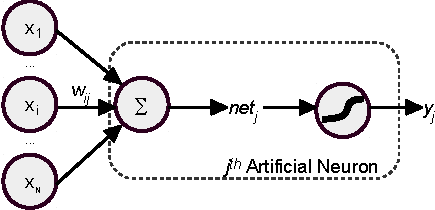
\includegraphics[width=0.7\textwidth]{pics_iconip/neuron.pdf}
	\caption{ $N$ neurons connect to the $j_{th}$ neuron of the next layer. As illustrated in Figure~\ref{Fig:compare_as}(a), we use \protect\TLSins{a} simplified artificial neuron without bias.}
	\label{Fig:neuron_net}
\end{figure}
Thus the gradient of the loss $L$ with respect to a weight $w_{ij}$ is as follows:
\begin{equation}
\begin{aligned}
\frac{\partial L}{\partial w_{ij}} &= \frac{\partial L}{\partial y_j} \frac{\partial y_j}{\partial net_j} \frac{\partial net_j}{\partial w_{ij}} = \delta_j x_i , \textrm{~~where~~}\\
 \delta_j &=  \frac{\partial L}{\partial y_j} \frac{\partial y_j}{\partial net_j}~~,  \textrm{~~and~~}\\
\frac{\partial net_j}{\partial w_{ij}} &= x_i~~.
\end{aligned}
\end{equation}
The term $ \delta_j $ represents the error gradient with respect to $net_j$, and can be expressed by a recursive definition:
\begin{equation}
\begin{aligned}
\delta_j =  \frac{\partial L}{\partial y_j} \frac{\partial y_j}{\partial net_j} &= \left\{
\begin{aligned}
&\frac{1}{K}\sum_{k=1}^K (y^{k}_{j}-t^{k}_{j}) f'(net_j)  \textrm{~,~~if \textit{j} is in an output layer} \\
&(\sum_l^L \delta_l w_{jl}) f'(net_j)  \protect\TLSdel{\textrm{~,~~if otherwise}}  \protect\TLSins{\textrm{~,~~otherwise}}
\end{aligned}
\right. \protect\TLSdel{\textrm{~,~~where}} \\\protect\TLSins{
\textrm{,~~where~~}} \frac{\partial y_j}{\partial net_j} &=  f'(net_j) \textrm{~,~~the derivative of the activation function}.
\end{aligned}
\label{equ:derivative}
\end{equation}
It is easy to obtain the first term, $ \frac{\partial L}{\partial y_j}  $, of $ \delta_j $ if $j$ is an output neuron since it only involves \protect\TLSins{a} single dimension of the output vector.
However, when $j$ is in an inner layer of the network, which connects \protect\TLSins{to} $L$ neurons on the next layer, we have to take \protect\TLSins{the} total derivative with respect to $y_j$: $\sum_l^L \delta_l w_{jl}$.
The error propagation applies to any form of connection in a network, such as FC and Conv layers, and the difference only appears in the summation where \protect\TLSins{the} matrix product is used for the FC layer and convolution for \protect\TLSins{the} Conv layer.
In addition, the weights used in BP are either transposed in \protect\TLSins{the} FC layer or rotated in \protect\TLSins{the} Conv layer compared to the forward path.

After error propagation, the BP algorithm updates weights using the optimisation method, gradient descent, to minimize the objective function.
It modifies the weights by small steps proportional to the negative of the gradients:
\begin{equation}
\Delta w_{ij} \propto -\frac{\partial L}{\partial w_{ij}} = -\eta \delta_j x_i~~,
\label{equ:delta_w}
\end{equation}
where $\eta$ defines the length of these updating steps which is also called \protect\TLSins{the} learning rate.
Again, the weight update is also \protect\TLSdel{dependant} \protect\TLSins{dependent} on the types of \protect\TLSdel{layers,} \protect\TLSins{layer,} where a convolution of the input vector $\mathbf{x}$ with the error gradient  $\mathbf{\delta}$ is needed in Conv layers.
A detailed description of BP training on \protect\TLSdel{ConvNet} \protect\TLSins{ConvNets} can be found \protect\TLSdel{in~.} \protect\TLSins{elsewhere~}\citep{bouvrie2006notes}\protect\TLSins{.}

Moreover, applying stochastic gradient descent (SGD), the gradient over the full training set can be approximated using only a single or a few training data.
Therefore $k$ in Equation~\ref{equ:derivative} can be seen as a randomly selected data index, and $K$ represents the number of elements in such a data subset, which is also known as a batch.
If we take only one data sample in each batch, the loss function~(Equation~\ref{equ:loss_all}) will be estimated by the error between an output vector $\mathbf{y}^k$ and the single label sample $\mathbf{t}^k$:
\begin{equation}
E^k = \frac{1}{2}\sum_{m=1}^M (y^{k}_{m}-t^{k}_{m})^{2}~~,
\label{equ:error_conv}
\end{equation}
and the equation can be simplified by deleting the index $k$, assuming the error is computed for each data sample:
\begin{equation}
E = \frac{1}{2}\sum_{m=1}^M (y_{m}-t_{m})^{2}~~.
\label{equ:error_non}
\end{equation}


\subsection{Activation Function and Vanishing Gradient}


\begin{figure}[tbp!]
	\centering
	\begin{subfigure}[t]{0.48\textwidth}
		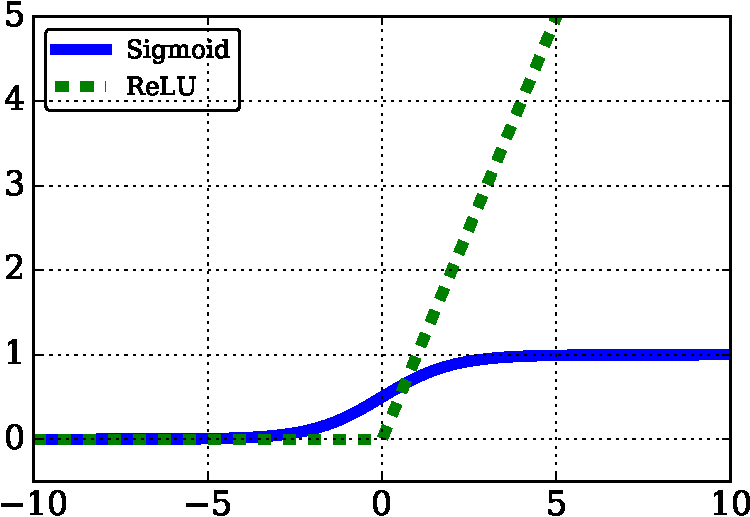
\includegraphics[width=\textwidth]{pics_snn/af.pdf}
		\caption{Activation functions}
	\end{subfigure}
	~~
	\begin{subfigure}[t]{0.48\textwidth}
		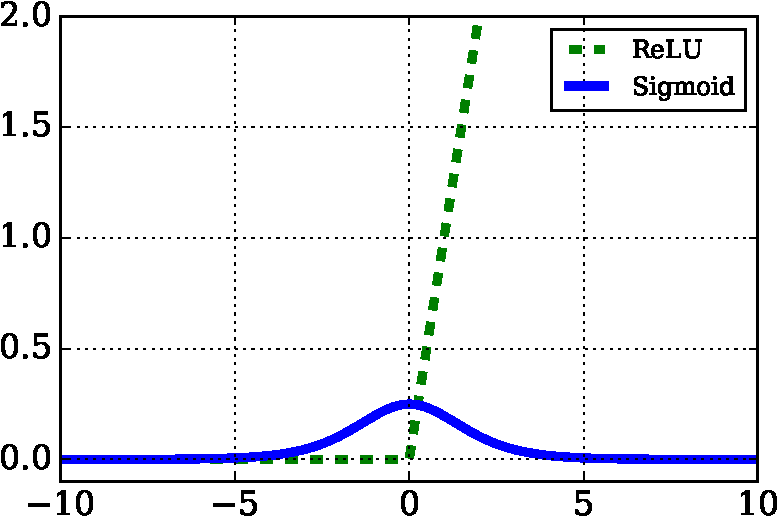
\includegraphics[width=\textwidth]{pics_snn/af_der.pdf}
		\caption{Derivatives of the activation functions}
	\end{subfigure}
	\caption{Activation functions: (a) sigmoid and ReLU, and (b) their derivatives.}
	\label{fig:af}
\end{figure}
Each error gradient propagated through layers of \protect\TLSins{the} network consists of a chain of multiplied factors as illustrated in Equation~\ref{equ:derivative}.
The deeper a network is and the closer a layer is to the input, the more elements are involved in the multiplication including the derivative of the activation function.
Thus, the gradient may vanish if the derivative of the activation function is always less than 1.
For the sigmoid function example, shown in Figure~\ref{fig:af}(a), \protect\TLSdel{its} \protect\TLSins{the} derivative \protect\TLSdel{keeps} \protect\TLSins{is} the maximum (around~0.25) only when the input is close to 0, and decays to its minimum 0 as the input either increases or decreases, see Figure~\ref{fig:af}(b).

\protect\TLSins{The} Rectified Linear Unit (ReLU) is proposed to tackle the problem of vanishing \protect\TLSdel{gradient} \protect\TLSins{gradients} in deep networks.
ReLU, simply defined as $y = max(0,x)$ and shown in Figure~\ref{fig:af}, has a gradient of 1 when the input is greater than 0.
Hence, the error gradient is able to be back-propagated in deeper network by multiplying ReLU derivatives.

\section{Autoencoders}
\label{sec:AE}
\protect\TLSdel{Autoencoders}
\protect\TLSins{Autoencoders~(AE)} are categorised as unsupervised \protect\TLSdel{learning,} \protect\TLSins{learning systems,} since AE aims to reconstruct its original input as closely as possible.
Thus the output and input vectors have the same \protect\TLSdel{dimensionality.
But} \protect\TLSins{dimensionality, but} the hidden middle layer is allowed to have either more, or fewer, neurons for the purpose of compressing the inputs or mapping them to higher dimensions.
Hence \protect\TLSins{the} AE is suitable \protect\TLSdel{to learn} \protect\TLSins{for learning an} effective representation of the original inputs at the hidden layer, which can be seen as the encoding phase of \protect\TLSins{the} AE, and \protect\TLSdel{reconstruct} \protect\TLSins{reconstructing} them on the output layer where the hidden vectors are decoded. 

Multiple AEs can be stacked to build deep AEs where the hidden layer of a lower AE represents the input of the upper block, and each AE block can be trained individually with greedy layer-wise training~\citep{hinton2006fast}.
A stacked AE takes advantage of greater expressive power as does any deep network.
Taking image processing as an example, the lower AE blocks learn only simple features, such as edges and dots, however on the upper layers more complicated and abstract features are extracted: contours, symbols and even objects. 

In this section, we will only describe the structure and training method of single AE blocks, since the greedy layer-wise training on stacked AEs is no different from training multiple single AEs except for different input data.
Due to \protect\TLSins{the} AE's simple network architecture and training algorithm, spiking AEs will be built and trained with \protect\TLSins{a} biologically-plausible training mechanism in Chapter~\ref{cha:sdlm}.

\subsection{Structure}
Figure~\ref{fig:AE} shows the architecture of an AE, which is an MLP consisting of three layers of neurons: \protect\TLSins{the} visible ($\mathbf{v}$), hidden ($\mathbf{h}$) and reconstruction ($\mathbf{v'}$) layers.
Both visible and reconstruction \protect\TLSdel{layer} \protect\TLSins{layers} have $N$ dimensions, and the hidden layer has $M$.
Note that AEs usually have tied weights where the connections ($\mathbf{w}^T$) between $\mathbf{v}$ and $\mathbf{h}$ are transposed to form the connections ($\mathbf{w}$) from $\mathbf{h}$ to $\mathbf{v'}$.


\begin{figure}
	\centering
	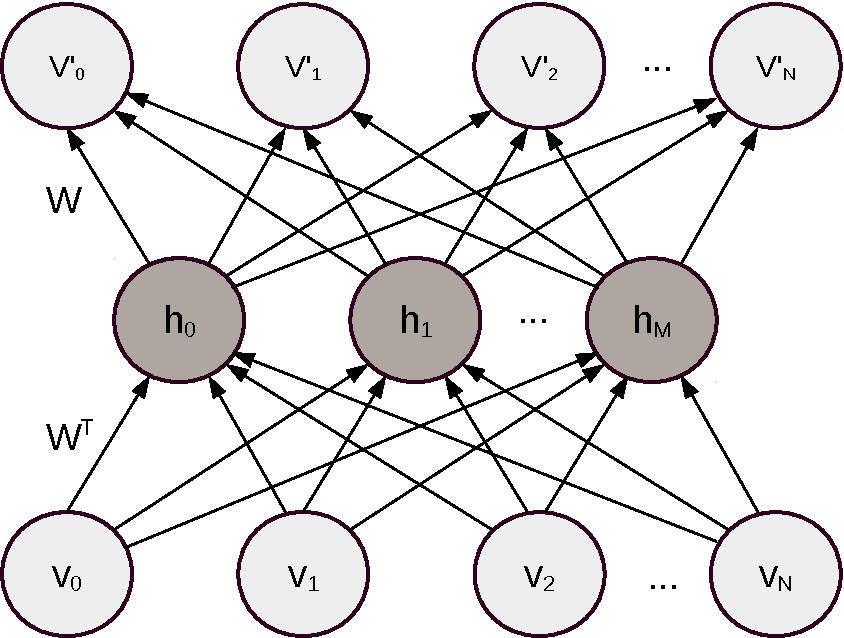
\includegraphics[width=0.5\textwidth]{pics_sdlm/AE.pdf}
	\caption{A typical Autoencoder structure.}
	\label{fig:AE}
\end{figure}


\subsection{Training}
The feedforward path of an AE, as for an MLP, non-linearly transforms the input through two FC layers, where each neuron performs weighted summation and activation as illustrated in Figure~\ref{Fig:neuron_net}.
Training an AE is also similar to that for an MLP, however, the difference lies in the objective where the AE aims to minimise the difference between the input $\mathbf{v}$ and its reconstruction $\mathbf{v'}$, instead of between the output and some labelled data (supervised learning).
Therefore the loss function generated by \protect\TLSins{a} single data sample $\mathbf{v}$, described in Equation~\ref{equ:error_non} for supervised learning, is as follow:
\begin{equation}
E = \frac{1}{2}\sum_{n=1}^N (v'_{n}-v_{n})^{2}~~,
\end{equation}
and the weight update, shown in Equation~\ref{equ:delta_w}, is proportional to the error gradient with respect to the weight:
\begin{equation}
\Delta w_{ij} \propto -\frac{\partial E}{\partial w_{ij}} = -\eta \delta_j h_i~~,
\end{equation}
where $\eta$ is the learning rate, $h_i$ is the hidden neuron and the term $\delta^k_j$ is the error gradient with the respect to $net_j$, the weighted summation.
The weight tuning needs only to be applied in the reconstruction layer, since study~\citep{xu1993least} has proved that updating the transposed weights $\mathbf{w}^T$ at the hidden layer does not improve the learning and the error gradients are usually small.
Hence, $\delta^k_j$  can be calculated according to Equation~\ref{equ:derivative}:
\begin{equation}
\delta_j = (v'_{j}-v_{j}) f'(net_j)~~,
\end{equation}
and the weight update can be simply described by:
\begin{equation}
\Delta w_{ij} = \eta h_i (v_{j}-v'_{j})  f'(net_j)~~.
\end{equation}
If we use ReLU as the activation function, then the above equation is as follow:
\begin{equation}
\label{equ:ae_widrow_hoff}
\Delta w_{ij} = \left \{
\begin{aligned}
& \eta h_i(v_j - v'_j)~, & net_j > 0 \\
& 0~, & net_j < = 0
\end{aligned} 
\right.
\end{equation}


\section{Restricted Boltzmann Machine}
\label{sec:rbm}
\protect\TLSdel{RBMs}
\protect\TLSins{The Restricted Boltzmann Machine~{RBMs}} share similar ideas of unsupervised learning with AEs, but aim to present a data distribution of some training dataset, rather than reconstructing each element of the dataset.
Thus, \protect\TLSins{the} RBM is an energy-based model and uses a stochastic approach.
Besides that, the structure of \protect\TLSdel{RBMs,} \protect\TLSins{an RBM,} see Figure~\ref{fig:RBM}, is also similar to \protect\TLSdel{AEs'} \protect\TLSins{an AE} where the visible units $\mathbf{v}$ bidirectionally connect to the hidden units $\mathbf{h}$ with strength $\mathbf{w}$.


\begin{figure}[hbt]
	\centering
	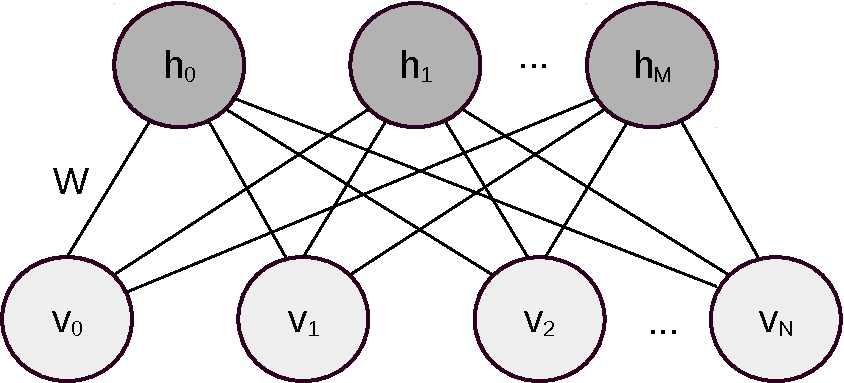
\includegraphics[width=0.6\textwidth]{pics_sdlm/rbm_o.pdf}
	\caption{A typical RBM structure.}
	\label{fig:RBM}
\end{figure}

Despite the various statistical models involved in RBMs and their training method, the actual training algorithm is rather simple thanks to the use of Contrastive Divergence~(CD)~\citep{hinton2002training}.
We can only illustrate some of the statistical models and sampling methods involved in RBM training, a detailed description can be found \protect\TLSdel{in~.} \protect\TLSins{elsewhere~}\citep{fischer2012introduction}\protect\TLSins{.} 
Stacked RBMs are also trained by layer-wise greedy algorithms, like stacked AEs, thus this section will focus on training a single RBM block.

\subsection{Energy-based Model}
In energy-based models, the probability of data point $x$ is defined by a model function $f(x)$, its energy function $E(x)$ and a partition function $Z$ which normalises the model function to possibilities by adding up all possible $f(x)$:
\begin{equation}
p(x) = \dfrac{f(x)}{Z}~~, \textrm{~~where~~} f(x) =e^{-E(x)}~~,  \textrm{~~and~~}
 Z = \sum_{x} e^{-E(x)}~~.
\end{equation} 
The energy function~\citep{hopfield1982neural} of \protect\TLSdel{a} \protect\TLSins{an} RBM is defined as follows:
\begin{equation}
E(\mathbf{v}, \mathbf{h} \mid \Theta)= -\sum_{i=1}^N a_i v_i - \sum_{j=1}^M b_j h_j - \sum_{i=1}^N \sum_{j=1}^M v_i w_{ij} h_j~~,
\label{equ:energy_complete}
\end{equation}
where the visible layer has $ N $ units, \protect\TLSins{the} hidden layer has $ M $, and $ \Theta$ are the model parameters used in RBMs $ \Theta =\{\mathbf{a}, \mathbf{b}, \mathbf{w}\} $ including biases on \protect\TLSins{the} visible layer, $\mathbf{a}$, \protect\TLSins{the} hidden \protect\TLSdel{layer, $\mathbf{b}$,} \protect\TLSins{layer $\mathbf{b}$} and weights between the layers $\mathbf{w}$.
As mentioned in Section~\ref{sec:spike}, for simplicity we use neurons without biases in this thesis.
Therefore only the third term of the complete energy function~(Equation~\ref{equ:energy_complete}) is kept:
\begin{equation}
E(\mathbf{v}, \mathbf{h} \mid \Theta)= - \sum_{i=1}^N \sum_{j=1}^M v_i w_{ij} h_j~~,
\label{equ:rbm_energy}
\end{equation}
and the model parameters are reduced to  $ \Theta = \{\mathbf{w}\} $.
Thus the joint probability of the visible vector (input) $\mathbf{v}$ and the output of \protect\TLSins{the} hidden units $\mathbf{h}$ is defined as follows: 
\begin{equation}
\begin{aligned}
p(\mathbf{v}, \mathbf{h} \mid \Theta) &=\frac{f(\mathbf{v}, \mathbf{h} \mid \Theta)}{Z(\Theta)}~,  \textrm{~where~} \\
f(\mathbf{v}, \mathbf{h} \mid \Theta) &=e^{-E(\mathbf{v}, \mathbf{h} \mid \Theta)}~,  \textrm{~and~} \\
Z(\Theta) &= \sum_{\mathbf{v}} \sum_{\mathbf{h}} e^{-E(\mathbf{v}, \mathbf{h} \mid \Theta)}~.
\end{aligned}
\label{equ:rbm_prob}
\end{equation}

\subsection{Objective Function}
Given a set of \protect\TLSdel{outcomes} \protect\TLSins{outcome} data $ \mathbf{D}=\{\mathbf{v}^1, \mathbf{v}^2, ..., \mathbf{v}^K\} $, the likelihood function of model parameters $\Theta$ defines the probability of the outcomes $ \mathbf{D}$ given $\Theta$:
\begin{equation}
L (\Theta \mid \mathbf{D}) = p(\mathbf{D} \mid \Theta ) = \prod_{k=1}^K p(\mathbf{v}^k \mid \Theta ) =  \prod_{k=1}^K\dfrac{f(\mathbf{v}^k \mid \Theta )}{Z( \Theta)}~~.
\label{equ:likelihood}
\end{equation}
Thus the objective is to maximise the likelihood $L (\Theta \mid \protect\TLSdel{\mathbf{D})$} \protect\TLSins{\mathbf{D})$;} that is to say, the model parameters $ \Theta $ \protect\TLSins{that} best \protect\TLSdel{defines} \protect\TLSins{define} the given data $\mathbf{D}$.
Furthermore, in order to simplify the product on the right-hand term in Equation~\ref{equ:likelihood} the objective function can be replaced with the average log-likelihood:
\begin{equation}
\label{equ:like}
\hat{l} (\Theta \mid \mathbf{D}) =\frac{1}{K}\log  L (\Theta \mid \mathbf{D}) 
=\frac{1}{K}\sum_{k=1}^K\log f(\mathbf{v}^k \mid \Theta ) - \log Z( \Theta)~~.
\end{equation}




The loss derivative with respect to a parameter $\theta$ is as follows:
\begin{equation}
\label{equ:part}
\begin{aligned}
\dfrac{\partial \hat{l} (\Theta \mid \mathbf{D})}{\partial \theta} 
& = \frac{1}{K} \dfrac{\partial \sum_{k=1}^K\log f(\mathbf{v}^k \mid \Theta )}{\partial \theta} - \dfrac{\partial \log Z( \Theta)}{\partial \theta}\\
& =  \frac{1}{K}\sum_{k=1}^K \dfrac{\partial \log f(\mathbf{v}^k \mid \Theta)}{\partial \theta} - \sum_x p(\mathbf{x} \mid \Theta) \dfrac{\partial \log f(\mathbf{x} \mid \Theta)}{\partial \theta}\\
& = \left \langle \dfrac{\partial \log f(\mathbf{v} \mid \Theta)}{\partial \theta}\right \rangle_{\mathbf{D}} -\left \langle \dfrac{\partial \log f(\mathbf{v} \mid \Theta)}{\partial \theta}\right \rangle_{\mathbf{C} \sim p(\mathbf{v} \mid \Theta)} ~~,
\end{aligned}
\end{equation}
where  $ <\cdot>_{\mathbf{X}} $ denotes the mean expectation of $ \cdot $ given data set $\mathbf{X}$.
The first term of the right-hand side is easy to get with the given data, $\mathbf{d} \in \mathbf{D} $, and the second term can be approximated by generating data samples $\mathbf{C} $ according to $ p(\mathbf{x} \mid \Theta) $.
The detailed derivation process can be found in Appendix~\ref{app:part}.
Applying the \protect\TLSins{RBM} model function \protect\TLSdel{of RBMs} in Equation~\ref{equ:rbm_prob} to the loss derivative (Equation~\ref{equ:part}), Appendix~\ref{app:RBM} derives the loss function of RBMs in detail:
\begin{equation}
\label{equ:RBM}
\begin{aligned}
\dfrac{\partial \hat{l} (\Theta \mid \mathbf{D})}{\partial \theta} 
& = \left \langle \dfrac{\partial -E(\mathbf{v}, \mathbf{h} \mid \Theta)}{\partial \theta} \right \rangle_{\{\mathbf{D}, \mathbf{D}_h\} \sim p( \mathbf{h} \mid \mathbf{v}, \Theta)} 
- \left \langle \dfrac{\partial -E(\mathbf{v}, \mathbf{h} \mid \Theta)}{\partial \theta} \right \rangle_{\{\mathbf{C_v}, \mathbf{C_h}\} \sim p( \mathbf{v}, \mathbf{h} \mid  \Theta)},  \\
\end{aligned}
\end{equation}
Then we plug the \protect\TLSins{RBM} energy function \protect\TLSdel{of RBMs} (Equation~\ref{equ:rbm_energy}) into the equation above, the loss derivative with respect to the weight is:
\begin{equation}
\label{equ:RBM_2}
\dfrac{\partial \hat{l} (\Theta \mid \mathbf{D})}{\partial w_{ij}} 
= \left \langle v_i h_j \right \rangle_{\{\mathbf{D}, \mathbf{D}_h\} \sim p( \mathbf{h} \mid \mathbf{v}, \Theta)}
- \left \langle  v_i h_j \right \rangle_{\{\mathbf{C_v}, \mathbf{C_h}\} \sim p( \mathbf{v}, \mathbf{h} \mid  \Theta)}~~. \end{equation}
\subsection{Weight update with Contrastive Divergence}
\label{sec:cd}
Generating data samples for the negative term of Equation~\ref{equ:RBM_2} requires Gibbs sampling on a Markov chain with \protect\TLSins{an} infinite \protect\TLSins{number of} steps to convergence.
Gibbs sampling approximates the joint probability $p( \mathbf{v}, \mathbf{h} \mid  \Theta)$ with \protect\TLSins{the} conditionally probability defined in RBMs:
\begin{equation}
\begin{aligned}
& p(h_j = 1 \mid \mathbf{v}) = \sigma(\sum_{i=1}^{M} w_{ij} v_i)~~,
& p(v_i = 1 \mid \mathbf{h}) = \sigma(\sum_{j=1}^{N} w_{ji} h_j)~~,
\end{aligned}
\label{equ:con_prob}
\end{equation} 
where $\sigma$ represents \protect\TLSins{the} Sigmoid activation function for Bernoulli-Bernoulli RBMs.
Figure~\ref{fig:gibbs} illustrates \protect\TLSdel{the} Gibbs sampling on an RBM by $k$ steps where each pair \protect\TLSdel{of} $(\mathbf{v}, \mathbf{h})$ composes a state of the Markov chain, and the joint probability $p( \mathbf{v}, \mathbf{h} \mid  \Theta)$ is approximated by conditional probabilities embedded in the weights (Equation~\ref{equ:con_prob}).

\begin{figure}[hbt]
	\centering
	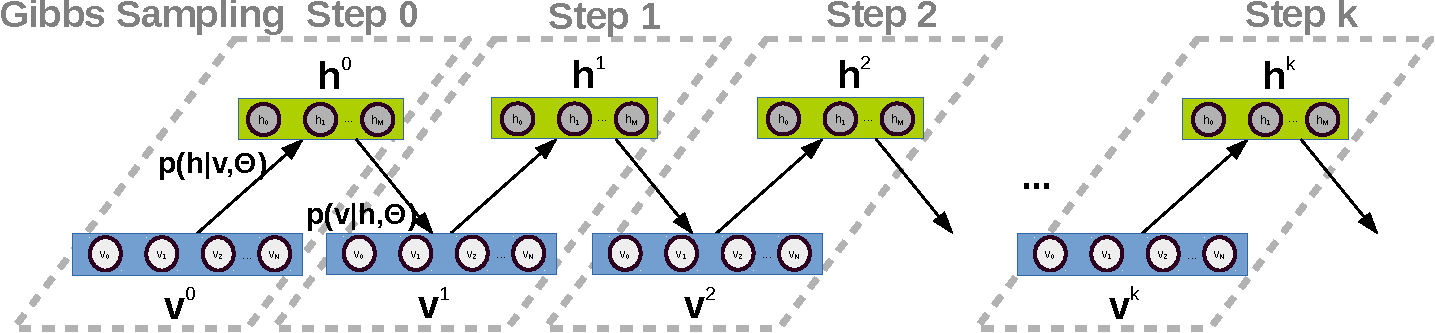
\includegraphics[width=0.98\textwidth]{pics_sdlm/gibbs_sampling.pdf}
	\caption{Gibbs sampling on \protect\TLSdel{a} \protect\TLSins{an} RBM.}
	\label{fig:gibbs}
\end{figure}

If $ k \to \infty $, the Markov chain will converge to an equilibrium which represents the distribution of the model-generated data $\{\mathbf{C_v}, \mathbf{C_h}\}$ described by the RBM, and Equation~\ref{equ:RBM} will represent the derivative of \protect\TLSins{the} Kullback-Leibler~(KL) divergence with respect to parameter $\theta$.
The KL divergence measures the distance between two probability distributions: the training dataset $\{\mathbf{D}, \mathbf{D_h}\}$ and the generated Gibbs samples, $\{\mathbf{C_v}, \mathbf{C_h}\}$.
However, if we \protect\TLSdel{just} take \protect\TLSins{just} a few steps, the KL divergence can be seen as a k-step contrastive convergence ($ CD_{k}) $.
Even $ CD_1 $ \protect\TLSdel{has performed} \protect\TLSins{performs} surprisingly well in RBM training~\citep{hinton2002training}.
Hence the RBM training using SGD is as follows :
\begin{equation}
\Delta w_{ij} = \eta (v^0_i h^0_j-v^1_i h^1_j)~~.
\label{equ:rbm_train}
\end{equation}




\section{Summary}
This chapter briefly introduced the most popular \protect\TLSdel{deep learning} \protect\TLSins{Deep Learning} techniques and models for potential use in spiking neural networks.
We illustrated the structure and training procedure for three \protect\TLSdel{deep learning} \protect\TLSins{Deep Learning} models: Convolutional networks, Autoencoders and Restricted Boltzmann Machines, which will be applied in spiking deep networks in the following chapters.